% Generated by tools/ca_figures.py from seed 11, flower 0. Do not edit.
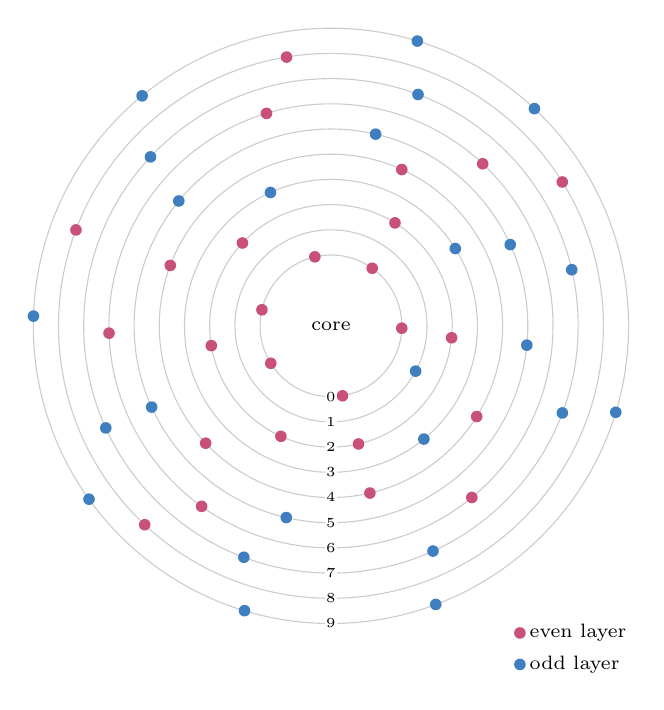
\begin{tikzpicture}[font=\scriptsize]
\definecolor{petA}{HTML}{C8507A}\definecolor{petB}{HTML}{3F7FBF}
\definecolor{petC}{HTML}{E0A030}\definecolor{petD}{HTML}{4E9A5B}
\definecolor{petE}{HTML}{8A5CB8}\definecolor{petF}{HTML}{D2693C}
\definecolor{petG}{HTML}{3AA6A0}\definecolor{petH}{HTML}{8C8C3A}
\draw[black!20] (0,0) circle (0.90);
\fill[petA] (103.12:0.90) circle (2.1pt);
\fill[petA] (279.38:0.90) circle (2.1pt);
\fill[petA] (358.12:0.90) circle (2.1pt);
\fill[petA] (211.88:0.90) circle (2.1pt);
\fill[petA] (166.88:0.90) circle (2.1pt);
\fill[petA] (54.38:0.90) circle (2.1pt);
\node[fill=white, inner sep=0.6pt] at (-90:0.90) {\tiny 0};
\draw[black!20] (0,0) circle (1.22);
\fill[petB] (331.88:1.22) circle (2.1pt);
\node[fill=white, inner sep=0.6pt] at (-90:1.22) {\tiny 1};
\draw[black!20] (0,0) circle (1.54);
\fill[petA] (189.38:1.54) circle (2.1pt);
\fill[petA] (136.88:1.54) circle (2.1pt);
\fill[petA] (58.12:1.54) circle (2.1pt);
\fill[petA] (283.12:1.54) circle (2.1pt);
\fill[petA] (354.38:1.54) circle (2.1pt);
\fill[petA] (245.62:1.54) circle (2.1pt);
\node[fill=white, inner sep=0.6pt] at (-90:1.54) {\tiny 2};
\draw[black!20] (0,0) circle (1.86);
\fill[petB] (309.38:1.86) circle (2.1pt);
\fill[petB] (31.88:1.86) circle (2.1pt);
\fill[petB] (114.38:1.86) circle (2.1pt);
\node[fill=white, inner sep=0.6pt] at (-90:1.86) {\tiny 3};
\draw[black!20] (0,0) circle (2.18);
\fill[petA] (328.12:2.18) circle (2.1pt);
\fill[petA] (159.38:2.18) circle (2.1pt);
\fill[petA] (223.12:2.18) circle (2.1pt);
\fill[petA] (283.12:2.18) circle (2.1pt);
\fill[petA] (65.62:2.18) circle (2.1pt);
\node[fill=white, inner sep=0.6pt] at (-90:2.18) {\tiny 4};
\draw[black!20] (0,0) circle (2.50);
\fill[petB] (354.38:2.50) circle (2.1pt);
\fill[petB] (76.88:2.50) circle (2.1pt);
\fill[petB] (256.88:2.50) circle (2.1pt);
\fill[petB] (140.62:2.50) circle (2.1pt);
\fill[petB] (204.38:2.50) circle (2.1pt);
\fill[petB] (24.38:2.50) circle (2.1pt);
\node[fill=white, inner sep=0.6pt] at (-90:2.50) {\tiny 5};
\draw[black!20] (0,0) circle (2.82);
\fill[petA] (181.88:2.82) circle (2.1pt);
\fill[petA] (309.38:2.82) circle (2.1pt);
\fill[petA] (106.88:2.82) circle (2.1pt);
\fill[petA] (46.88:2.82) circle (2.1pt);
\fill[petA] (234.38:2.82) circle (2.1pt);
\node[fill=white, inner sep=0.6pt] at (-90:2.82) {\tiny 6};
\draw[black!20] (0,0) circle (3.14);
\fill[petB] (294.38:3.14) circle (2.1pt);
\fill[petB] (13.12:3.14) circle (2.1pt);
\fill[petB] (136.88:3.14) circle (2.1pt);
\fill[petB] (69.38:3.14) circle (2.1pt);
\fill[petB] (249.38:3.14) circle (2.1pt);
\fill[petB] (339.38:3.14) circle (2.1pt);
\fill[petB] (204.38:3.14) circle (2.1pt);
\node[fill=white, inner sep=0.6pt] at (-90:3.14) {\tiny 7};
\draw[black!20] (0,0) circle (3.46);
\fill[petA] (99.38:3.46) circle (2.1pt);
\fill[petA] (31.88:3.46) circle (2.1pt);
\fill[petA] (159.38:3.46) circle (2.1pt);
\fill[petA] (226.88:3.46) circle (2.1pt);
\node[fill=white, inner sep=0.6pt] at (-90:3.46) {\tiny 8};
\draw[black!20] (0,0) circle (3.78);
\fill[petB] (129.38:3.78) circle (2.1pt);
\fill[petB] (343.12:3.78) circle (2.1pt);
\fill[petB] (215.62:3.78) circle (2.1pt);
\fill[petB] (178.12:3.78) circle (2.1pt);
\fill[petB] (290.62:3.78) circle (2.1pt);
\fill[petB] (46.88:3.78) circle (2.1pt);
\fill[petB] (73.12:3.78) circle (2.1pt);
\fill[petB] (253.12:3.78) circle (2.1pt);
\node[fill=white, inner sep=0.6pt] at (-90:3.78) {\tiny 9};
\node[align=center] at (0,0) {core};
\fill[petA] (2.4,-3.9) circle (2.1pt) node[right, black] {even layer};
\fill[petB] (2.4,-4.3) circle (2.1pt) node[right, black] {odd layer};
\end{tikzpicture}
